%!TEX root = ./main.tex
\chapter{Mackey Functors} % (fold)
\label{cha:mackey_functors}
参考文献有:\cite{li-2015}

\section{Introduction} % (fold)
\label{sec:introduction}
\begin{figure}[htbp]
	\centering
	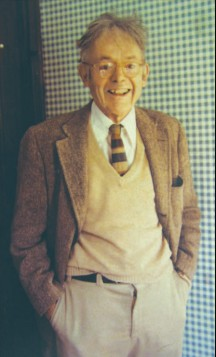
\includegraphics[width=0.3\textwidth]{./figures/Mackey.jpg}
	\caption{George Mackey}
\end{figure}
George W. Mackey (1916–2006) was an American mathematician. For more interesting story about him, see \url{https://en.wikipedia.org/wiki/George_Mackey}, \url{http://www.ams.org/notices/200707/tx070700824p.pdf} or \url{http://www-history.mcs.st-andrews.ac.uk/Biographies/Mackey.html}. And I found an interesting fact that Leslie Lamport's advisor Richard Palais was a PhD student of him.\footnote{\url{http://www.genealogy.ams.org/id.php?id=35871}} And Lamport is best known for the system \LaTeX.\footnote{\url{https://en.wikipedia.org/wiki/Leslie_Lamport}}


Mackey functor is an algebraic structure, related to many constructions from finite groups, such as group cohomology and the algebraic $K$-theory of group rings.

History: began in 1980s\\
People:  Dress and Green first gave the axiomatic formulation of Mackey functors.
% section introduction (end)







% chapter mackey_functors (end)